%-------------------------
% Resume in Latex
% Based off of: https://github.com/sb2nov/resume
% and Jake Gutierrez's version of it
% at https://www.overleaf.com/latex/templates/jakes-resume/syzfjbzwjncs
% inspired by https://practicaltypography.com/resumes.html
% License : MIT
%------------------------

\documentclass[a4paper,11pt]{article}

\usepackage{latexsym}
\usepackage[empty]{fullpage}
\usepackage{titlesec}
\usepackage{marvosym}
\usepackage[usenames,dvipsnames]{xcolor}
\usepackage{verbatim}
\usepackage{enumitem}
\usepackage[hidelinks]{hyperref}
\usepackage[margin = 1in]{geometry}
\usepackage{fancyhdr}
\usepackage[english]{babel}
\usepackage{tabularx}
\usepackage{wrapfig}
\usepackage{graphicx}

%--------------UNDERLINING---------------
% taken from https://alexwlchan.net/2017/10/latex-underlines/

\usepackage{contour}
\usepackage{ulem}

\renewcommand{\ULdepth}{3.8pt}
\contourlength{0.8pt}

\newcommand{\myuline}[1]{%
  \uline{\phantom{#1}}%
  \llap{\contour{white}{#1}}%
}

%----------------------------------------

\graphicspath{ {./Images/} }

%----------FONT OPTIONS----------
\usepackage{fontspec}
\usepackage{fontawesome5}

% I could have just used the charter package here for the font I wanted...
% but I'd still need to change compiler to XeLaTeX to include the title font
% \usepackage{charter}

\setmainfont{XCharter}

\newfontfamily{\basictitle}{basictitlefont}[
Path = Fonts/,
Extension = .ttf,
UprightFont = basictitlefont
]
% to use:
% {\basictitle This text uses the basictitle font}

\pagestyle{fancy}
\fancyhf{} % clear all header and footer fields
\fancyfoot{}
\renewcommand{\headrulewidth}{0pt}
\renewcommand{\footrulewidth}{0pt}

% Adjust margins
\iffalse
% \iftrue
\addtolength{\oddsidemargin}{0.3in}
\addtolength{\marginparsep}{0.3in}
\addtolength{\evensidemargin}{0.3in}
\addtolength{\textwidth}{-0.5in}
\addtolength{\topmargin}{0.3in}
\addtolength{\textheight}{0.3in}
\fi

\urlstyle{same}

\raggedright
\setlength{\tabcolsep}{0in}

% Sections formatting
\titleformat{\section}{
    {\color{gray}\titlerule} \vspace{-5pt}
    \vspace{8pt}\scshape\raggedright\normalfont
}{}{0pt}{}

%-------------------------
% Custom commands
\newcommand{\resumeItem}[1]{
  \item\small{
    {#1 \vspace{-2pt}}
  }
}

\newcommand{\resumeSubheading}[4]{
  \vspace{-2pt}\item
    \begin{tabular*}{0.97\textwidth}[t]{l@{\extracolsep{\fill}}r}
      \textbf{#1} & #2 \\
      \textit{\small#3} & \textit{\small #4} \\
    \end{tabular*}\vspace{-7pt}
}

\newcommand{\resumeSubSubheading}[2]{
    \item
    \begin{tabular*}{0.97\textwidth}{l@{\extracolsep{\fill}}r}
      \textit{\small#1} & \textit{\small #2} \\
    \end{tabular*}\vspace{-7pt}
}

\newcommand{\resumeProjectHeading}[2]{
    \item
    \begin{tabular*}{0.97\textwidth}{l@{\extracolsep{\fill}}r}
      \small#1 & #2 \\
    \end{tabular*}\vspace{-7pt}
}

\newcommand{\resumeSubItem}[1]{\resumeItem{#1}\vspace{-4pt}}

\renewcommand\labelitemii{$\vcenter{\hbox{\tiny$\bullet$}}$}

\newcommand{\resumeSubHeadingListStart}{\begin{itemize}[leftmargin=0.15in, label={}]}
\newcommand{\resumeSubHeadingListEnd}{\end{itemize}}
\newcommand{\resumeItemListStart}{\begin{itemize}}
\newcommand{\resumeItemListEnd}{\end{itemize}\vspace{-5pt}}

%-------------------------------------------
%%%%%%  RESUME STARTS HERE  %%%%%%%%%%%%%%%%%%%%%%%%%%%%


\begin{document}

% ----- TOGGLE PHOTO --------
% comment out \iffalse and remove the % from \iftrue to toggle photo
\iffalse
% \iftrue
\begin{wrapfigure}{R}{0.15\textwidth}
\vspace{-35pt}
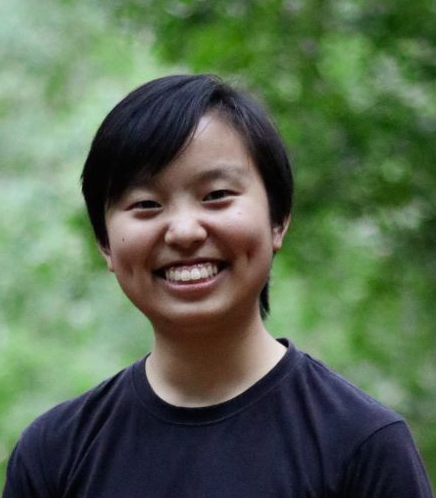
\includegraphics[scale=0.20]{dp_cropped}
\end{wrapfigure}
\fi

%----------HEADING----------

{\basictitle \Huge Arthur Goldblatt}
\\

% ----- TOGGLE FOR PHOTO ----
% \vspace{10pt}

\href{mailto:arthurgoldblatt@berkeley.edu}{
    \faEnvelope
    \thinspace \thinspace
    \myuline{arthurgoldblatt@berkeley.edu}} $|$
\href{https://www.linkedin.com/in/arthur-goldblatt-39719285/}{
    \faLinkedin
    \thinspace \thinspace        
    \myuline{arthur-goldblatt}} $|$
\href{https://github.com/arthurgoldblatt}{
    \faGithub
    \thinspace \thinspace
    \myuline{arthurgoldblatt}} $|$
\faPhone
\thinspace \thinspace
(510)295-3358

%-----------EDUCATION-----------
\section{Education}
  \resumeSubHeadingListStart
    \resumeSubheading
      {University of Berkeley, California}{Berkeley}
      {B. Eng. Electrical Engineering and Computer Science}{Aug. 2017 -- May 2021}
      \resumeItemListStart
      
        \resumeItem{3.79 GPA}

      \resumeItemListEnd
      
  \resumeSubHeadingListEnd
  
    %-----------PROJECTS-----------
\section{Coding Projects}
    \resumeSubHeadingListStart
      \resumeProjectHeading
          {\href{https://github.com/hkrsmk/beepboop-shopee-code-league-2020}{\myuline{\textbf{Shopee Code League}}} $|$ \textit{Python, Jupyter Notebooks, Google Cloud Platform}}{June -- Aug 2020}
          \resumeItemListStart
            \resumeItem{Set up data pipeline: Kaggle > cloud storage > Google Colab Notebooks\\for faster analysis}
            \resumeItem{Set up github repository for team}
          \resumeItemListEnd
    \resumeSubHeadingListEnd


%-----------EXPERIENCE-----------
\section{Experience}
  \resumeSubHeadingListStart
  
    \resumeSubheading
      {Analyst}{May 2020 -- Present}
      {ALLFED - Alliance to Feed the Earth in Disasters}{Remote, part-time}
      \resumeItemListStart
        \resumeItem{Final year project}
        \resumeItem{Research on global catastrophic risks and how they affect industry}
        \resumeItem{Aim to answer this question: If all of our electricity grids shut down for 5 years or more, how can we preserve industry and infrastructure such that we can resume industry as quickly as possible?}
      \resumeItemListEnd

    \resumeSubheading
      {Research Associate}{Feb -- Mar 2020}
      {DouxMatok}{Petach Tikva, Israel}
      \resumeItemListStart
        \resumeItem{Synthesised sugars with new additives using vacuum mixers}
        \resumeItem{Proposed new research protocol to test food products}
        \resumeItem{Prepared rheology calibration curves}
      \resumeItemListEnd
      
    \resumeSubheading
      {Research Assistant}{Jul 2019 -- Jan 2020}
      {Cuberg Inc.}{Emeryville, CA, USA}
      \resumeItemListStart
        \resumeItem{Worked in the glovebox: built 412 coin cells, synthesised 125 electrolytes}
        \resumeItem{Created and upgraded three critical tools in Google sheets and Jupyter notebooks for better data analysis, which automated previously-manual processes}
        \resumeItem{Built battery testing equipment (software and hardware)}
        \resumeItem{Conducted  a human subject study to determine which video game dungeon generation technique is enjoyable}
        \resumeItem{Wrote an 8-page paper and gave multiple presentations on-campus}
        \resumeItem{Presented virtually to the World Conference on Computational Intelligence}
      \resumeItemListEnd
      
      \iffalse
      % \iftrue
% -----------Multiple Positions Heading-----------
    \resumeSubSubheading
     {Software Engineer I}{Oct 2014 - Sep 2016}
    \resumeItemListStart
        \resumeItem{Apache Beam}
          {Apache Beam is a unified model for defining both batch and streaming data-parallel processing pipelines}
     \resumeItemListEnd
    \resumeSubHeadingListEnd
%-------------------------------------------

    \fi

    \resumeSubheading
      {ESG Data Analyst}{May -- Aug 2018}
      {Schneider Electric}{Singapore}
      \resumeItemListStart
        \resumeItem{Optimised usage of in-house energy monitoring software and reaped energy savings of \$1,545 per month}
        \resumeItem{Created 12 other mini-deliverables; 10 were self-initiated. These include databases, guides, and reports, along with internal learning materials for EcoStruxure, Schneider Electric’s main product offer}
        \resumeItem{Founded the Singapore branch’s Green Committee}
        \resumeItem{Organised Global Environment Day activities for the staff}
      \resumeItemListEnd
      
      \iffalse
      % \iftrue
    \resumeSubheading
      {Consultant}{Feb 2017}
      {National Environment Agency}{Singapore}
      \resumeItemListStart
        \resumeItem{Reviewed 4 candidate topics for R\&D funding: found current research grants and current environment technology}
      \resumeItemListEnd
      
    \resumeSubheading
      {Innovation Consultant}{Dec 2016}
      {Land Transport Authority}{Singapore}
      \resumeItemListStart
        \resumeItem{Proposed folding seat solution increases train capacity by 13\%}
        \resumeItem{Achieved best presentation award (out of 9 pairs of people)}
      \resumeItemListEnd
\fi

  \resumeSubHeadingListEnd

%-----------RESEARCH-----------
\section{Research (papers linked)}
  \resumeSubHeadingListStart
  
    \resumeSubheading
      {\href{https://drive.google.com/open?id=1mmfRboc6VkFRZTedy0Wzz4gklM4_84w3}{\myuline{Rechargeable aqueous zinc batteries}}}{Aug 2018 -- Jun 2019}
      {with Prof Srinivasian Madhavi}{NTU, Singapore}
      \resumeItemListStart
        \resumeItem{Synthesised electrolytes, ran CVs \& three-electrode tests}
        \resumeItem{Published results in URECA (undergrad research) proceedings}
      \resumeItemListEnd
      
    \resumeSubheading
      {\href{https://drive.google.com/open?id=1U78X1NCEEXN3O1o8Wnd_czyM6F7XEFJh}{\myuline{Lithium ion battery anodes}}}{Dec 2017 -- May 2018}
      {with Prof Srinivasian Madhavi}{NTU, Singapore}
      \resumeItemListStart
        \resumeItem{Synthesised battery slurries}
        \resumeItem{Learned various techniques: XRD analysis, cyclic voltammetry, thermogravimetric analysis, hydrothermal synthesis, data analysis}
        \resumeItem{Published paper in ChemElectroChem (third author)}
        \begin{itemize}
            \item DOI: 10.1002/celc.201801244
        \end{itemize}
      \resumeItemListEnd
      
    \resumeSubheading
      {Dye-sensitised Solar Cells}{Apr -- Jul 2017}
      {with Associate Prof Soo Han Sen}{NTU, Singapore}
      \resumeItemListStart
        \resumeItem{Tested 4 experiment variables and conditions}
        \resumeItem{Increased scale of synthesis by 20\%}
      \resumeItemListEnd

  \resumeSubHeadingListEnd

%-----------CCAs-----------
\section{Extracurriculars}
    \resumeSubHeadingListStart
    
      \resumeSubheading
      {Founder}{Jan 2018 -- present}
      {Breathe Easy NTU/Hazy Waste}{}
      \resumeItemListStart
        \resumeItem{Won \$5,000 grant to promote sustainable palm oil in Singapore}
        \resumeItem{Lead a team of 18 to \href{https://drive.google.com/file/d/1SHm7c42NkIvISBImdOo7QajR64gDjuw9/view}{\myuline{survey 237 students}} and \href{https://drive.google.com/file/d/1Y2rG_mDPt50KHoXztLaMhA1Tjk7pM_7E/view?usp=sharing}{\myuline{44 canteen vendors}} for their view on palm oil, producing 2 reports on the results}
        \resumeItem{Converted one canteen to sustainable palm oil; NUS followed suit}
      \resumeItemListEnd
    
      \resumeSubheading
          {Operations}{Jul 2018 -- Present}
          {Effective Altruism Singapore}{}
          \resumeItemListStart
            \resumeItem{Set up scalable Eventbrite ticketing platform with Zapier integration}
            \resumeItem{Facilitate inaugural Arete Fellowship in Singapore for Asia}
          \resumeItemListEnd
          
      \resumeSubheading
      {External Liaison Director}{Aug 2018 -- May 2019}
      {Earthlink NTU}{}
      \resumeItemListStart
        \resumeItem{Lead a team of 3 to organise 3 events and run 3 booths, with total turnout of 450 across the 6}
      \resumeItemListEnd
      
      \resumeSubheading
      {Assistant Head}{Jul 2018 -- Jul 2019}
      {ASEAN Youth Organization}{}
      \resumeItemListStart
        \resumeItem{Organised the ASEAN Youth Conference for roughly 100 ASEAN participants in an international team of 17}
      \resumeItemListEnd
          
    \resumeSubHeadingListEnd

\iffalse
%-----------PROGRAMMING SKILLS-----------
\section{Skills}
 \begin{itemize}[leftmargin=0.15in, label={}]
    \small{\item{
     \textbf{Languages}{: Python, C/C++, SQL, JavaScript, HTML/CSS, R} \\
     \textbf{Developer Tools}{: Jupyter Notebooks, Git, Google Cloud Platform, VS Code, Amazon AWS} \\
     }
     }
     }
 \end{itemize}
 \fi


%
%\iffalse
\iftrue
%-----------PROGRAMMING SKILLS-----------
\section{Technical Skills}
 \begin{itemize}[leftmargin=0.15in, label={}]
    \small{\item{
     \textbf{Languages}{: Python, C/C++, SQL, JavaScript, HTML/CSS, R} \\
     \textbf{Frameworks}{: WordPress} \\
     \textbf{Developer Tools}{: Jupyter Notebooks, Git, Google Cloud Platform, VS Code, Amazon AWS} \\
     \textbf{Libraries}{: pandas, plotly}
    }}
 \end{itemize}
\fi

%-------------------------------------------
\end{document}
